\documentclass{article}
\usepackage{epsfig, latexsym}

\begin{document}

\newcommand{\SOPmin}{${\rm SOP}_{\rm min} \ $}
\newcommand{\POSmin}{${\rm POS}_{\rm min} \ $}
\newcommand{\bs}{\backslash}


\title{
\Huge{CMPEN 270 -- Fall 2015}\\
\normalsize{Return this exam!  No calculators!}\\
\normalsize{Exam 1}\\
\makebox[4in][l]{Name:} }
\date{}

\maketitle{}


\begin{enumerate}

\item {\bf (2 pts.)} Convert $101000_2$ to decimal.

\begin{tabular}{p{0.7in} p{0.7in} p{0.7in} p{0.7in} l}
a)20 & b)24  & c)40  & d)42  & e) none of the above
\end{tabular}

\item {\bf (2 pts.)} Convert $42_{10}$ to binary.

\begin{tabular}{p{0.7in} p{0.7in} p{0.7in} p{0.7in} l}
a) $010010_2$ & b) $100010_2$ & c) $100110_2$ & d) $100100_2$ & e) none of the above
\end{tabular}

\item {\bf (2 pts.)} Convert $42_{16}$ to binary.

\begin{tabular}{p{0.7in} p{0.7in} p{0.7in} p{0.7in} l}
a) $1000010_2$ & b) $1000100_2$ & c) $1000110_2$ & d) $1001000_2$ & e) none of the above
\end{tabular}

\item {\bf (2 pts.)} How many bits do you need to represent the number 48?

\begin{tabular}{p{0.7in} p{0.7in} p{0.7in} p{0.7in} l}
a) 4  & b) 5 & c) 6 & d) 7 & e) none of the above
\end{tabular}

\item {\bf (1 pts.)} When representated as 4-bit binary numbers does 12 + 4
generate overflow?

\begin{tabular}{p{0.7in} l}
a) yes & b) no  c) Trick question, 12 cannot be represented in 4-bit
\end{tabular}


\item {\bf (2 pt.)} Which expression is equivalent to (A'+B)'(B+AC)?
\begin{description}
\item{a) } 0
\item{b) } 1
\item{c) } AB'C
\item{d) } AB' + AB'C
\item{e) } None of the above
\end{description}

\pagebreak

\underline{For questions 7-10 let F(A,B,C)= A'B + A(B'+ BC')}

\item {\bf (2 pts.)} What does F(0,1,0) equal?

\begin{tabular}{p{0.7in} p{0.7in} p{0.7in} p{0.7in} l}
a) 0 & b) 1 & c) C & d) C' & e) none of these
\end{tabular}

\item {\bf (1 pts.)} What does F(1,1,C) equal?

\begin{tabular}{p{0.7in} p{0.7in} p{0.7in} p{0.7in} l}
a) 0 & b) 1 & c) C & d) C' & e) none of these
\end{tabular}

\item {\bf (2 pt.)} How many AND gates does it take to realize F
as is (do not simplify)?

\begin{tabular}{p{0.7in} p{0.7in} p{0.7in} p{0.7in} l}
a) 1 & b) 2 & c) 3 & d) 4 & e) none of these
\end{tabular}

\item {\bf (2 pt.)} How many OR gates does it take to realize F
as is (do not simplify)?

\begin{tabular}{p{0.7in} p{0.7in} p{0.7in} p{0.7in} l}
a) 1 & b) 2 & c) 4 & d) 5 & e) none of these
\end{tabular}

\underline{Utilize the following truth table for problems 11 and 12.}

\begin{tabular}{c|c|c||c|c}
A & B & C & F & G \\ \hline \hline
0 & 0 & 0 & 1 & 1 \\ \hline
0 & 0 & 1 & 0 & 0 \\ \hline
0 & 1 & 0 & 0 & 0 \\ \hline
0 & 1 & 1 & 0 & 1 \\ \hline
1 & 0 & 0 & 1 & 1 \\ \hline
1 & 0 & 1 & 1 & 0 \\ \hline
1 & 1 & 0 & 0 & 1 \\ \hline
1 & 1 & 1 & 0 & 1 \\
\end{tabular} 

\item {\bf (2 pt.)} What function is described by $\prod M(0,3,4,6,7)$?

\begin{tabular}{p{0.7in} p{0.7in} p{0.7in} p{0.7in} l}
a) F & b) F' & c) G & d) G' & e) none of the above
\end{tabular}

\item {\bf (2 pt.)} How many sum terms does the canonical POS expression 
for F have?

\begin{tabular}{p{0.7in} p{0.7in} p{0.7in} p{0.7in} l}
a) 1 & b) 2 & c) 3 & d) 4 & e) 5
\end{tabular}

\item {\bf (3 pts.)} How many different \SOPmin solutions exist for \\
F(A,B,C)=$\Sigma$m (1,3,4,5,6) ?

\begin{tabular}{p{0.7in} p{0.7in} p{0.7in} p{0.7in} l}
a) 1 & b) 2 & c) 3 & d) 4 & e) 5
\end{tabular}

$ \begin{array} {c||c|c|c|c}
        A \bs BC & 00 & 01 & 11 & 10 \\ \hline \hline
        0        &    &    &    &    \\ \hline
        1        &    &    &    &    \\ 
\end{array} $


\pagebreak

\underline{Utilize the following word statement for problems 14 and 15.}


Design a 4-input $a_1a_0b_1b_0$, two output $o_1 o_0$ digital circuit.  
$A=a_1a_0$ and $B=b_1b_0$ represent 2-bit binary numbers.  The output 
is the smaller of $A$ and $B$.  For example, if $A=10$ and $B=01$, then $O=01$.

\item {\bf (2 pt.)}How many rows of the truth table have $O_1 = 1$?

\begin{tabular}{p{0.7in} p{0.7in} p{0.7in} p{0.7in} l}
a) 1 & b) 4 & c) 9 & d) 12 & e) None of the above.
\end{tabular}

\item {\bf (2 pt.)}How many rows of the truth table have $O_0 = 0$?

\begin{tabular}{p{0.7in} p{0.7in} p{0.7in} p{0.7in} l}
a) 1 & b) 4 & c) 9 & d) 12 & e) None of the above.
\end{tabular}

\item {\bf (1 pt.)}A grouping of 4 cells generates a product term with 4 
variables.  How many variables does the kmap have?

\begin{tabular}{p{0.7in} p{0.7in} p{0.7in} p{0.7in} l}
a) 3 & b) 4 & c) 5 & d) 6 & e) None of the above.
\end{tabular}


\marginpar{ \tiny $$ 
\begin{array}{c|c|c|c||c|c}
a_1 & a_0 & b_1 & b_0 & o_1 & o_0 \\ \hline
0 & 0 & 0 & 0 &   &    \\ \hline
0 & 0 & 0 & 1 &   &    \\ \hline
0 & 0 & 1 & 0 &   &    \\ \hline
0 & 0 & 1 & 1 &   &    \\ \hline
0 & 1 & 0 & 0 &   &    \\ \hline
0 & 1 & 0 & 1 &   &    \\ \hline
0 & 1 & 1 & 0 &   &    \\ \hline
0 & 1 & 1 & 1 &   &    \\ \hline
1 & 0 & 0 & 0 &   &    \\ \hline
1 & 0 & 0 & 1 & 0 & 1  \\ \hline
1 & 0 & 1 & 0 &   &    \\ \hline
1 & 0 & 1 & 1 &   &    \\ \hline
1 & 1 & 0 & 0 &   &    \\ \hline
1 & 1 & 0 & 1 &   &    \\ \hline
1 & 1 & 1 & 0 &   &    \\ \hline
1 & 1 & 1 & 1 &   &    \\
\end{array}$$
{\rm Truth Table for }O }


\vspace{0.5in} 

\underline{For questions 17,18 use the figure below.}

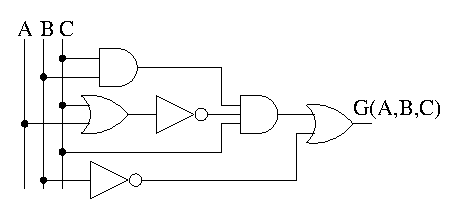
\includegraphics{./Fig1/cir_5}


\item {\bf (2 pt.)} What is the symbolic representation of $G(A,B,C)$
(do not simplify).
\begin{description}
\item{a) } BC + (A + C)' + B'
\item{b) } BC(A+C)' + B'
\item{c) } BC(A+C)'C + B'
\item{d) } B'
\item{e) } None of the above.
\end{description}

\item {\bf (2 pt.)} What is G(1,1,0)=?
\begin{description}
\item{a) } 1
\item{b) } 0
\end{description}

\pagebreak

\marginpar{ \tiny $$ 
\begin{array} {c||c|c|c|c}
        AB \bs CD & 00 & 01 & 11 & 10 \\ \hline \hline
        00        &    &    &    &    \\ \hline
        01        &    &    &    &    \\ \hline
        11        &    &    &    &    \\ \hline
        10        &    &    &    &    \\
\end{array} $$}

\item {\bf (3 pts.)} Determine the \SOPmin expression for \\
F(A,B,C,D)=$\sum m(0,1,5,6,7,8,9,14)$

\begin{description}
\item{a) }A'B'C' + A'BD + BCD' + AB'C'
\item{b) }B'C' + A'BD + BCD'
\item{c) }A'C'D + BCD' + B'C'
\item{d) }B'C'D' + B'C'D + A'BD + BCD'
\item{e) } None of the above.
\end{description}

\marginpar{ \tiny $$ 
\begin{array} {c||c|c|c|c}
        AB \bs CD & 00 & 01 & 11 & 10 \\ \hline \hline
        00        &    &    &    &    \\ \hline
        01        &    &    &    &    \\ \hline
        11        &    &    &    &    \\ \hline
        10        &    &    &    &    \\
\end{array} $$}

\item {\bf (3 pt.)} Determine the \SOPmin expression for \\
F(A,B,C,D)=$\Sigma$m(1,2,3,7,8,9,11,15)

\begin{description}
\item{a) } A'B'D + A'B'C + ACD + AB'C'D' + AB'CD'
\item{b) } A'B'C + AB'C'+ B'D + CD
\item{c) } A'B'C + A'BD + AB'C'+ AB'D + CD
\item{d) } A'B' + AB' + CD
\item{e) } None of the above.
\end{description}

\marginpar{ \tiny $$ 
\begin{array} {c||c|c|c|c}
        AB \bs CD & 00 & 01 & 11 & 10 \\ \hline \hline
        00        &    &    &    &    \\ \hline
        01        &    &    &    &    \\ \hline
        11        &    &    &    &    \\ \hline
        10        &    &    &    &    \\
\end{array} $$}

\item {\bf (4 pt.)} Determine the \POSmin expression for \\
F(A,B,C,D)= (A+B'+D)(B+C')(B'+C'+D)

\marginpar{ \tiny $$ 
\begin{array} {c||c|c|c|c}
        AB \bs CD & 00 & 01 & 11 & 10 \\ \hline \hline
        00        &    &    &    &    \\ \hline
        01        &    &    &    &    \\ \hline
        11        &    &    &    &    \\ \hline
        10        &    &    &    &    \\
\end{array} $$}

\begin{description}
\item{a) } (B+C')(A+B'+D')(C'+D)
\item{b) } (B+C'+D')(C'+D)(A+B'+D)
\item{c) } (A+B'+D)(B+C')(B'+C'+D)
\item{d) } (B+C)(A'+C)(B'+D)
\item{e) } None of the above.
\end{description}

\marginpar{ \tiny $$ 
\begin{array} {c||c|c|c|c}
        AB \bs CD & 00 & 01 & 11 & 10 \\ \hline \hline
        00        &    &    &    &    \\ \hline
        01        &    &    &    &    \\ \hline
        11        &    &    &    &    \\ \hline
        10        &    &    &    &    \\
\end{array} $$}

\item {\bf (3 pt.)} Determine the \SOPmin expression for \\
F(A,B,C,D)= A'D+BD+AC'D'+AB'D

\begin{description}
\item{a) } A + D
\item{b) } AC' + D
\item{c) } AC'D' + D
\item{d) } AC'D + A'D + AB
\item{e) } None of the above.
\end{description}

\end{enumerate}

\end{document}


